%% ---------------------------------------------------------------
%% $URL: https://repository.cs.ru.is/svn/thesis-template/trunk/ruthesis/latex/DEGREE-NAME-YEAR.tex $
%% $Id: DEGREE-NAME-YEAR.tex 311 2016-10-04 11:04:16Z foley $
%% This is a template LaTeX file for theses or reports at Reykjavík University
%% Particularly the Computer Science or Science and Engineering departments
%% The template and ruthesis.cls file have been designed to be compatible with
%%   LaTeX, PDFTeX, and XeTeX.
%% 
%% Comments and questions can be sent to 
%% General: the RU LaTeX group (latex AT list.ru.is) 
%% Computer Science: the Graduate Study Council (cs-grad AT ru.is)
%% Science and Engineering: graduate administrator: Kristín Kristinsdóttir (kristinkri AT ru.is)
%% See the README for information on final preparation for PhD Dissertations
%%
%% Original Author: Bjórn Þór Jónsson (bjorn AT ru.is)
%% Modified by: Eyjólfur Ingi Ásgeirsson <eyjo AT ru.is>
%% Modified and Maintained by: Joseph Timothy Foley <foley AT ru.is>
%% ---------------------------------------------------------------

%% METHOD:
%% 0) Read README.TXT
%% 0.1) !!!NO REALLY, READ README.TXT!!!
%% 0.2) Subscribe to the announcements email list at
%%    https://list.ru.is/mailman/listinfo/latex-announcements
%% 1 LaTeX instructions.tex or goto http://afs.rnd.ru.is/project/thesis-template/trunk/ruthesis/latex/instructions.pdf
%% 2) Copy the template (or unzip) to your working area
%% 3) Rename this file (if needed) with your information e.g. MSC-FOLEY-2007.tex
%% 4) Modify this file to fit your needs (please follow all comments below in the text)
%% 5) For making bibliographies, run "biber".  You can also change
%% this back to "bibtex".  See below in "Bibliography options".

%% Options for ruthesis class:

%%%%%%% CHOOSE ONE OF THESE %%%%%%%%%%%%%%%
%% projectreport: Project report (CS)
%% bachelors: Bachelor of Science thesis
%% masters: Master of Science thesis
%% doctorate: Doctor of Philosophy dissertation
%%
%%%%%%% CHOOSE ONE OF THESE %%%%%%
%% 
%% draft: speed up processing by skipping graphics and adding useful
%%     information for editing.  Also sets spacing to double so that it is easier   %%     to write editing marks on paper copy.
%% proof:  proofreading version (final formatting with warnings)
%% final: generate document for submission, removing FIXMEs, and
%%     other markup.  Throw error if any fatal FIXMEs still in document.
%%
%%%%%%%% CHOOSE ANY COMBINATION OF THESE %%%%%%%%%%%%
%%
%% booklet: set the stock/font size for booklets (experimental, DO NOT USE)
%% forcegraphics: force graphics, etc. to be included, even in draft mode
%% debug:  writes more messages to the log file, adds debugging output 
%%     and sizing boxes
%% miktex: disable some packages that cause problems for (older) MikTeX
%% icelandic: thesis is in Icelandic
%% oldstyle:  use the PhD headers and footers from the old CS template
%% online: for online versions (skip additional signature pages)
\documentclass[masters,forcegraphics,miktex,draft]{ruthesis}

%%%%%%% HACKS:  USE THESE ONLY IF INSTRUCTED TO DO SO!!!! %%%%%%%%%%%%%%%
%% yngvihack:  Proposed changes to the template from Dean Yngvi
%\setboolean{yngvihack}{true}

%% Note, if you are writing a PhD thesis, it will be reduced at the
%% printers when it is bound into a book: B5 240x170mm (aka Programme
%% or Book economy) See the README.TXT for details.  Plan your figures
%% and diagrams for this size.  In a future release of this template,
%% setting booklet will allow you to see what it would look like.

%% For other thesis, print them out in A4, then they will be cut down
%% to 293x206mm by the binder.  Make sure you use "acid-free" paper or
%% the book will yellow and fall apart in a few years.
%% TODO: instructions to the printer about bleed

%%%%%%%%%%%%%%%%%%%% TeXStudio Magic Comments %%%%%%%%%%%%%%%%%%%%%
%% These comments that start with "!TeX" modify the way TeXStudio works
%% For details see http://texstudio.sourceforge.net/manual/current/usermanual_en.html   Section 4.10
%%
%% What encoding is the file in?
% !TeX encoding = UTF-8
%% What language should it be spellchecked?
% !TeX spellcheck = en_US
%% What program should I compile this document with?
% !TeX program = pdflatex
%% Which program should be used for generating the bibliography?
% !TeX TXS-program:bibliography = txs:///biber
%% This also sets the bibliography program for TeXShop and TeXWorks
% !BIB program = biber

%%%%%%%%%%%%%%%%%%%% Bibliography options %%%%%%%%%%%%%%%%%%%%%
%% We suggest switching from bibtex to biblatex/biber because it is better able
%% to deal with Icelandic characters and other bibliography issues
%% As long as you use biblatex instead of bibtex by itself, it will at least
%%  generate a document without errors.
%% !!!If you are using TeXStudio, don't forget to update the bibliography setting!!!
\usepackage[backend=biber,bibencoding=utf8,style=ieee]{biblatex}
%\DeclareLanguageMapping{american}{american-apa}  
% need to declare mapping for style=apa to alphabetize properly
% If you set backend=bibtex, it will use bibtex for processing (old way)
%    this can work with Icelandic characters, but you may get weird results.
%    bibtex does not know how to sort Þ and ð
% if you set backend=biber, you can use UTF8 characters such as Þ and
%     ð  but you will have to remember to switch from using bibtex to 
%     biber in your client
% If you use JabRef, make sure the file is encoded in UTF-8 which is
%    not the default.

%% This tells TeXStudio to use biber
% !TeX TXS-program:bibliography = txs:///biber

% Where is your reference library?
\addbibresource{references.bib}

%%%%%%%%%%%%%%%%%%% CUSTOMIZATIONS %%%%%%%%%%%%%%%%%%%%%%%%%%%%%
%% It is not recommended that you customize this file
%%   nor ruthesis.cls.   You should put your macros and packages into
%%   a separate file so that it is easier to use updates to the template.
%% The custom.tex file was created for this reason.
%% We load this much later so that it can overrite any existing settings
\InputIfExists{custom.tex}

%%%%%%%%%%%%%%% INFORMATION %%%%%%%%%%%%%%%%%%5
%% University information must be multilingual to deal with the
%%  required cover pages and abstract on thesis
%% NOTE: This may not be required for other reports!!!

%% Babel Icelandic macros are setup  on RedHat at
%% /usr/share/texlive/texmf-dist/tex/generic/babel/icelandic.sty
%% /usr/share/texlive/texmf-dist/tex/generic/babel-icelandic/icelandic.ldf


%% Multilingual macros
%\newML{macroname}{englishword}{icelandicword}
%  creates \macronameML
%    \MLmacroname[english] - returns the english word
%    \MLmacroname[icelandic] - returns the icelandic word
%    \MLmacroname  - uses the current language setting
% Some useful ones have already been defined, but can be redefined
%% Predefined: \MLIceland \MLReykjavikUniversity \MLUniversityIceland

%% What institute?  Default is RU.
%\setInstitution{\MLReykjavikUniversity}
% \newML{InstitutionAddress}{Menntavegur 1\\101 Reykjavík, Iceland}
% {Menntavegi 1\\101 Reykjavík, Ísland}
% \setInstitutionAddress{\MLInstitutionAddress}
% \newML{Tel}{Tel.}{Sími}
% \setInstitutionPhone{\MLTel{} +354 599 6200\\
% Fax +354 599 6201}
% \setInstitutionURL{www.ru.is}


%% Department and degree program

%% School of Computer Science: \MLCS
% Programs:  Computer Science, Software Engineering, Language Technology
%\program{Computer Science}

%% School of Science and Engineering \MLSSE
%% Programs: 
%% Bioinformatics, Biomedical Engineering
%% Civil Engineering with specialization in Concrete Technology
%% Civil Engineering with specialization in Construction Management
%% Civil Engineering with specialization in Structural Design
%% Civil Engineering with specialization in Transport and Urban Planning
%% Construction Management
%% Electrical Engineering
%% Mechatronics
%% Engineering Management
%% Exercise Science and Coaching
%% Financial Engineering
%% Mechanical Engineering
%% Sustainable Energy Engineering - REYST
%% Sustainable Science - REYST
%% Urban Planning and Transport

\setSchool{\MLSSE}
\newML{program}{Electrical Engineering}{Electrical Engineering}
\program{\MLprogram}

%% Degree long name.  If not already defined, you can create a macro
%\newML{DEGREE}{English Degree Name}{Icelandic Degree Name}
%% Default is set based upon doctorate vs masters option
%% Predefined: \MLMSc \MLPhd
%\setDegreelong{\MLMSc}

%% Degree abb, change if default is not right
%% Default is set based upon doctorate vs masters option
%\degreeabbrv{Sc.D.} 


%\setFrontLogo{reyst-logo}
%% Use this if you need a different front logo on the first page
%% e.g. reyst-logo

%% Date in english and icelandic
%% NOTE: THIS IS THE DATE OF THE SUPERVISOR'S SIGNATURE!!!!!!
%% Predefined: \MLjan, \MLfeb, \MLmar, ... \MLdec
%\whensigned{day}{month}{year} %day is only used on some formats, but you must put something.
\whensigned{10}{\MLmay}{2018}

%% Title in english and icelandic
%% This is required on Thesis, but not necessarily elsewhere.
%%
%% Note that title length is limited to what can fit in three lines in the inside page
%% Also note that the capitalization of the text on the front page is a potential source
%% of latex errors as it may not deal well with math, international letters, 
%% and other latex constructs
%% Warning: capitalization does not always work anyway
\newML{Title}{Smart Micro-controller Based Integrated Monitoring and Protection System for Three-Phase Power Transformer}{Örtölvu Byggt Öryggis og Eftirlitskerfi fyrir Þriggja Fasa Spennubreytir}
%\newML{Title}{Working Title}
\newML{TITLE}{WORKING TITLE}{TITLL VERKEFNIS}
%% If you have the title in just one language, put it into \setTitle{} directly e.g.
%%  \setTitle{Working Title}
%%
\setTitle{\MLTitle}
%% If you need to adjust the main title later, you can use
%% \setMainTitle{}
%% ***** Special Titles ******
%% If the title must be formatted specifically for the cover page or internal pages
%% (typically via line-breaks using the \newline command) then the following commands must be used 
%%
%% This one for the online/PhD front page:
%%  and should usually be kept short per line
%% The template specified that a PhD cover should have the title in capitals, but
%%  the physical copies have not done this.  This macro is in case that
%%  turns out to be important
%\setTitleCover{\MLTITLE}
%% These two for the internal cover pages, usually not needed
%\newML{TitleInternal}{Internal Title}{Icelandic Internal Title}
%\setTitleInternal{\MLTitleInternal}

%% Author name (should be the same in any language, if not use \newML)
%% If you are writing a Project report with multiple authors, separate them with \\:
%% To keep the names typeset together, you want to use non-breaking spaces
%% TODO: fix formatting for TVD BSc multi-author (x4) --foley
%\author{Firstname1~Lastname1\\Firstname2~Lastname2}
\author{Kristján Guðmundur~Birgisson}

%% If the name must be formatted specifically for the signature page
%% (typically via line-breaks) then the following command must be used 
%\setAuthorSignature{Student\\Name}
%% This macro adjusts the author name in the headers of the oldstyle formatting
%\setAuthorHeader{StudentLast}

%%%%%%%%%%%%%%%%%%%%%%%%%% Project Report or Bachelor's Only!!! %%%%%%%%%%%%%%%%%%%%%%%%%%%%%%%%%%%%%%%%%%%
\setCourse{VT LOK 1012}

%%%%%%%%%%%%%%%%%%%%%%%%%% Project Report Only!!! %%%%%%%%%%%%%%%%%%%%%%%%%%%%%%%%%%%%%%%%%%%


%%%%%%%%%%%%%%%%%%%%%%%%%% Bachelors Only!!! %%%%%%%%%%%%%%%%%%%%%%%%%%%%%%%%%%%%%%%%%%%
\setID{280489--2559}%kennitala
\setSemester{2017--8}
\setShortSignedDate{1.1.2016}

\setOrganization{Háskólinn í Reykjavík.\\Menntavegur 1\\ Reykjavík}
\setSubProgram{Tæknifræði}

%% If the thesis is confidential, uncomment this with the date it can be released
%\setClosedDistribution{10.1.2016}%

%% Put your keywords here in English, then Icelandic.  Separate them with commas.
\newML{keywords}{Keyword1, Keyword2, Keyword3}{Lykliorð1, Lykliorð2, Lykliorð3}
\setKeywords{\MLkeywords}

%%%%%%%%%%%%%%%%%%%%%%%%%%% Masters Only!! %%%%%%%%%%%%%%%%%%%%%%%%%%%%%%%%%%%%%%%%%%%%
%% How many credits (ECTS) on Master's degree
%% Usually 30 or 60
\ects{60}

%%%%%%%%%%%%%%%%%%%%%%%%%%% Doctorate Only!! %%%%%%%%%%%%%%%%%%%%%%%%%%%%%%%%%%%%%%%%%%
%% Some Computer Science Thesis have an ISSN number.
%% Most other documents do not.
%\bookidnumber{ISSN: 1670-8539} 
%% ID numbers are optional, but nice for sorting in libraries

%% International Standard Book Number (ISBN)
%% This is what most people should use if the thesis is being published.

%% International Standard Serial Number (ISSN)
%% This is usually only for a PhD dissertation as part of a series when published
%%   Computer Science: 1670-8539 

%% Additional degrees?  (optional, usually not needed)
%\adddegree{(list of degrees in appendix)}{(sjá lista yfir prófgraður í viðauka)}
%%%%%%%%%%%%%%%%%%%%%%%%%%%%%%%%%%%%%%%%%%%%%%%%%%%%%%%%%%%%%%%%%%%%%%%%%%%%%%%%%%%%%%%%


%% List the entire committee.  Each member has a name (degree should be omitted, unless it is not PhD),
%% Supervisor(s) must appear first
%% On a Bachelors, there is usually only one supervisor and one examiner.

%% Format for each entry:
%%  \personinfo{Name}{Role}{Job Title}{Company/institution}{Country}
%% Predefined macros: \MLSupervisor \MLSupervisors \MLExaminer \MLExaminers

%% Change these to singular/plural as needed.
%% Just uncomment and change the plurality of the macro.
%\setSupervisorHeading{\MLSupervisors}
%\setExaminerHeading{\MLExaminer}

%% Predefined macros:
%% \MLSeniorProfessor \MLProfessor \MLAssociateProfessor \MLAdjunctProfessor \MLEmeritusProfessor \Iceland
%% \MLReykjavikUniversity \MLUniversityIceland

%% Bachelors: primary advisor (Umsjónarkennari), ONLY ONE!
%% All others: As many as you want
\supervisors{
  \personinfo{Mohammed Abdelfattah}{\MLSupervisor}{\MLProfessor}{\MLReykjavikUniversity}{\MLIceland}
%  \personinfo{Helpful A. Teacher}{Co-advisor}{\MLAssistantProfessor}{\MLUniversityIceland}{\MLIceland}
%  \personinfo{Ian M. Great}{Co-advisor}{\MLProfessor}{Hochschule Düsseldorf}{Germany}
}

%% Bachelors: secondary advisor (Leiðbeinandi), ONLY ONE
%% All others: As many as you want
\examiners{
  \personinfo{Tough E. Questions}{\MLExaminer}{Associate Professor}{Massachusetts Institute of Technology}{USA}

}

%% An abstract is required to be in both Icelandic and English for most degrees.
%% It is considered good form to limit the abstract to a single paragraph in each language,
%%   around 250 words or so.  Refer to your degree's instructions.
%% Note: Icelandic quotation marks cannot be typeset using "` and "'.  You should use \enquote{}
%%   this is probably due to interactions with the MultiLingual macros.
\newML{AbstractText}{\lipsum[1]}  
% ipsum generaes text text
{\lipsum[1]} % Icelandic abstract goes here
\setAbstract{\MLAbstractText}


%%%%%%%%%%%%%%INDEX SETUP %%%%%%%%%%%%%%%%%%%%%%%%%%%%%%%%%%%%%%%%%%%%%%%%%%%%
%% Indexes, and other auto-generated material
%% The Memoir package (which we use) automatically generates the index
%% information but you need a program to put them back into the document
%% This means you have to run "makeindex DEGREE-NAME-YEAR"
%% !!!Do not load any of the index packages, they cause problems with Memoir!!!
%% !!!You have been warned!!!
\makeindex

%% For abbreviations, you may want to try
%% Watch out though, each new index writes another external file and 
%% latex can only write a limited number of them
%%\usepackage[intoc]{nomencl} % intoc: In Table of Contents
%% remember to run:
%% makeindex filename.nlo  -s nomencl.ist -o filename.nls

\finalifforcegraphics{hyperref} %hyperlinks even in draft mode
\usepackage[hidelinks]{hyperref} 
%% !!!Must be the last package loaded except otherwise mentioned!!!!
%% \usepackage{hypcap}  %% puts link at top of figure, must be after hyperref

%%%%%%%%%%%%%GLOSSARY SETUP%%%%%%%%%%%%%%%%%%%%
%% A glossary is a nice thing to have in larger documents.
%% Unfortunately, it seems to cause problems on many TeX installations
%%  so it is disabled by default.
%% Uncomment the lines that start with \% in order to re-enable it

% % add an autogenerated glossary (separate from main index)
%% Warning: package glossaries doesn't like it when they are defined in the document
%% http://mirror.ctan.org/macros/latex/contrib/glossaries/glossaries-user.html#sec%3adocdefs
%%
%% WARNING!  Memoir has an internal "index" option which conflicts with glossaries
%% Loading the package must go after hyperref (it is special).
%\RequirePackage[acronym,toc]{glossaries}
%% nomain: no main glossary
%% acronym: acronym glossary
%% toc: add entry in Table of Contents
%% automake: try to run makeindex using \write18 shell escape
%% without automake, run "makeglossaries" to process them
%% or the right makeindex options
%\makeglossaries{}  % intitialize the glossary.  Must be in the main file!!!
%%% $URL$
%% $Id$
%% Glossary term definitions
%% Note, you will need to reference them in the text after defining them

\newglossaryentry{glossary}{name=glossary, description={a place to put all the terms that confuse people}}
\newglossaryentry{ohm}{name=ohm,symbol={\ensuremath{\Omega}}, description=unit of electrical resistance}  % Do not break this with newlines!
\newglossaryentry{dissertation}{name=dissertation, description={A large pile of paper that professors use to prop up shelves.}}
\newacronym{rfid}{RFID}{Radio Frequency IDentification}

\newacronym{led}{LED}{light-emitting diodes}

\newacronym{auv}{AUV}{Autonomous Undersea Vehicle}
%% Reference manual: http://ctan.uib.no/macros/latex/contrib/glossaries/glossaries-user.pdf

%% You can also define most entries near where they are used, but this may cause problems.  See manual chapter 4.8
%% Be careful about putting entries on Chapter, Section, etc.  See manual Chapter 6.



%%% Local Variables: 
%%% mode: latex
%%% TeX-master: "DEGREE-NAME-YEAR"
%%% End: 
  % load glossary definitions in preamble

%%%%%%%%%%%%%%%%%%%%%%%%%%%%%%%%%%%%%%%%%%%%%%%%%%%%%%%%%%%%%%%%%%%%%%%%%%
%%%%%%%%%%%%%%%%%%%%%%% DOCUMENT START %%%%%%%%%%%%%%%%%%%%%%%%%%%%%%%%%%%

\begin{document}
%% Some elements have different names on the RU Masters rules
%% They will be annotated with RUM: "name"
\frontmatter{} % setup formatting at beginning

\frontcover{}%% The MSc/BSc cover can be gotten from the front desk and has a window in it
%%RUM: Front cover (standard)
\frontrequiredpages{}  % the various signature pages

\ifdraft{\coverchapter{Important!!!  Read the Instructions!!!} If you
  have not already done so, \LaTeX{} the \path{instructions.tex} to
  learn how to setup your document and use some of the features.  You
  can see a (somewhat recent) rendered PDF of the instructions at
  \url{http://afs.rnd.ru.is/project/thesis-template/trunk/ruthesis/latex/instructions.pdf}.
  There is also more information on working with \LaTeX{} at
  \url{http://afs.rnd.ru.is/project/htgaru/trunk/how-to-get-around-projects.pdf}.
  This includes common problems and fixes.

  This page will disappear in anything other than draft mode.}{}



\newML{child}{child}{barn}  
%% Dedication is optional, comment out if it is absent
%% RUM: Not mentioned
\begin{dedications}
  I dedicate this to my spouse/\MLchild{}/pet/power animal.
\end{dedications}

\enableindents{}% turn on/off paragraph indents
% RUM: "Acknowledgements (optional)"
\coverchapter{Acknowledgements} 
\begin{quotation}
So long, and thanks for all the fish.
\end{quotation}\sourceatright{Douglas Adams}%\cite{adams84fish}}
\vspace{\baselineskip}

\draftnote{Acknowledgements are optional; comment this chapter out if they are absent
  Note that it is important to acknowledge any funding that helped in the work}

This work was funded by \the\year~RANNIS grant ``Survey of man-eating Minke whales'' 1415550.
Additional equipment was generously donated by the Icelandic Tourism Board.

\coverchapter{Preface}
% RUM: "Preface (optional)"
This dissertation is original work by the author, Firstname~Lastname.
Portions of the introductory text are used with permission from
Student et al.%\cite{student2015awesome} of which I am an author.

  
\draftnote{The preface is an optional element
  explaining a little who performed what work.  See
  \url{https://www.grad.ubc.ca/sites/default/files/materials/thesis_sample_prefaces.pdf}
  for suggestions.
  
  List of publications as part of the preface is
  optional unless elements of the work have already been published.
  It should be a comprehensive list of all publications in which
  material in the thesis has appeared, preferably with references to
  sections as appropriate.  This is also a good place to state
  contribution of student and contribution of others to the work
  represented in the thesis.}


%\coverchapter{Publications}
%% RUM: Not mentioned, this was found in the CS thesis template.  
%% Maybe more applicable to PhD dissertations?
%%% Probably a duplication from before Preface became standard.


\starttables{} % setup formatting
%% TOC, list of figures and list of tables are required
\tableofcontents{}%%RUM: "Table of contents"
\thesislistoffigures{}%%RUM: "List of figures"
\thesislistoftables{}%%RUM: "List of tables"

%\coverchapter{List of drawings and enclosed material}
%RUM: "List of drawings and enclosed material, e.g. CD(as appropriate)"

\listoffixmes{}
% if using fixme package, lists what needs to be done

%% The list of abbreviations is an example of a special list
%% Other lists may be added, such as lists of algorithms, symbols, theorems, etc.
%% IN CS PhD, this is sometimes centered.
\newtoclist{Abbreviations}%%RUM: Not mentioned
\begin{tabular}{ll}
MSc &Masters of Science\\
PhD &Doctor of Philosophy\\
kV  &kilo Volt\\
DC	&Direct Current\\
AC	&Alternative Current\\
HV	&High Voltage\\
LV	&Low Voltage \\
HC	&High Current\\
LC	&Low Current\\
CT	&Current Transformer\\
GT	&Generator Transformer\\
ST	&Station Transformer\\
DT	&Distribution Transformer\\
UAT	&Unit Auxiliary Transformer\\
AT	&Auxiliary Transformer\\
IT	&Instrument Transformer\\
RT	&Rectifier Transformer\\
NGT	&Neutral Ground Transformer\\
ANSI	&American National Standards Institute\\
M-C	&Micro Controller
\end{tabular}

\newtoclist{Symbols}%%RUM: Not mentioned
\begin{tabular}{lll}
Symbol &Description &Value/Units\\
$V$ &Voltage &\si{Volt}\\
$A$ &current &\si{I}	\\
$c$ &Speed of Light &\SI{2.99E8}{\meter\per\second\square}\\
\end{tabular}

%% This command prepares for the actual text, e.g. by 
%% calling \mainmatter{}
\starttext{}

%% ---------------------------------------------------------------
%% From this point on, it is standard Latex, except the very end.
%% This is a "report"-based template, so the top-level heading 
%% is \chapter{}

%% WARNING: Make sure that all of these files (and any new ones)
%% are UTF-8 otherwise you will get weird encoding errors.
%\part{The First Part} % Parts optional but useful in longer documents

%% The default division is IMRAD, you may want to divide differently
%% See the introduction for guidance.

%% This file only is included if we are draft mode.
%% The instructions.tex file contains instructions and examples.
%\ifdraft{\documentclass[projectreport,online,forcegraphics,miktex,draft]{ruthesis}
\usepackage[backend=biber,bibencoding=utf8,style=ieee]{biblatex}
\addbibresource{references.bib}
\InputIfExists{custom.tex}
\setTitle{Writing a Thesis in \LaTeX{}}
%% Because datetime is broken, we always have to set a \whensigned{day}{MLmonth}{year}
\whensigned{12}{\MLdec}{2016}
\author{Joseph Timothy Foley}
\setCourse{Final Project Reports, Thesis, and Dissertations}
\setSchool{\MLSSE{} \& \MLSCS{}}

%% Making glossaries needs perl installed
%% Usually only Windows needs this installed separately
%% http://www.activestate.com/activeperl
%\RequirePackage[acronym,toc]{glossaries}
\RequirePackage[toc]{glossaries}
%% nomain: no main glossary
%% acronym: acronym glossary
%% toc: add entry in Table of Contents
%% automake: try to run makeindex using \write18 shell escape
%% without automake, run "makeglossaries" to process them
%% or the right makeindex options
%\newglossary[slg]{symbols}{sym}{sbl}{List of Symbols}
\makeglossaries{}  % intitialize the glossary.  Must be in the main file!!!
%% $URL$
%% $Id$
%% Glossary term definitions
%% Note, you will need to reference them in the text after defining them

\newglossaryentry{glossary}{name=glossary, description={a place to put all the terms that confuse people}}
\newglossaryentry{ohm}{name=ohm,symbol={\ensuremath{\Omega}}, description=unit of electrical resistance}  % Do not break this with newlines!
\newglossaryentry{dissertation}{name=dissertation, description={A large pile of paper that professors use to prop up shelves.}}
\newacronym{rfid}{RFID}{Radio Frequency IDentification}

\newacronym{led}{LED}{light-emitting diodes}

\newacronym{auv}{AUV}{Autonomous Undersea Vehicle}
%% Reference manual: http://ctan.uib.no/macros/latex/contrib/glossaries/glossaries-user.pdf

%% You can also define most entries near where they are used, but this may cause problems.  See manual chapter 4.8
%% Be careful about putting entries on Chapter, Section, etc.  See manual Chapter 6.



%%% Local Variables: 
%%% mode: latex
%%% TeX-master: "DEGREE-NAME-YEAR"
%%% End: 
  % load glossary definitions in preamble

%% You get indexes for free from the memoir package.  Don't use anything else!
%% You have been warned!
\makeindex

\finalifforcegraphics{hyperref} %hyperlinks even in draft mode
\usepackage[hidelinks]{hyperref} 


\begin{document}
\frontmatter{}
\frontcover{}
\enableindents{}

\starttables{} % setup formatting
%% TOC, list of figures and list of tables are required
\tableofcontents{}%%RUM: "Table of contents"
\thesislistoffigures{}%%RUM: "List of figures"
\thesislistoftables{}%%RUM: "List of tables"
\starttext{}
%\coverchapter{List of drawings and enclosed material}
%RUM: "List of drawings and enclosed material, e.g. CD(as appropriate)"

\listoffixmes{}
% if using fixme package, lists what needs to be done

\chapter{Getting started}
\section{Introduction}
Before using the template in \path{DEGREE-NAME-YEAR.tex}, the author
recommends reading the (in progress) guide to successful projects,
including \LaTeX{} at
\url{http://afs.rnd.ru.is/project/htgaru/trunk/how-to-get-around-projects.pdf}.
Full instructions on setting up \LaTeX{} and SubVersion are there.
Additionally, as issues are discovered, they are added to the
Frequently Asked Questions section in that document.

Text will be double spaced when in draft mode so that there is room
for reviewers to write comments.  Extra blank pages are also removed.
If you want to check formatting in a more final form, switch to
proofing mode.  This text in gray will disappear when you are not in
draft mode.  It is better to use FiXme's as a reminder mechanism,
though.  See Section~\ref{sec:fixme}

\textbf{WARNING} It is very very important that you print the generated PDF at 100\% scaling.   
On many computers, printing is set to adjust the size to fit the page.
Do not do this, because it will mess up the sizes of the font and the placement of the letters.
This becomes very evident when you print it out and the cover window does not line up with your title!

\section{Citing properly}
Any content from external sources must be properly cited.
If any part of this document is plagiarized (from another group,
the internet, or anywhere else) or your references are not properly
cited, you will be in a lot of trouble.

This is in compliance with Reykjavík University's Code of
Ethics\footnote{\url{http://en.ru.is/the-university/ru-code-of-ethics/}
  -- see Item 8 and General Rules on Study and Examinations}
\footnote{\url{http://en.ru.is/studies/study--and-examination-rules/}
  -- see Article 4.5} \footnote{see also the document "Your Work -
  Your Contribution" \url{http://www.ru.is/hugverk}, available only in
  Icelandic}. For your reference, here is a link to guidelines
defining plagiarism and discussing how to avoid it (from the
University of Oxford):

\url{http://www.ox.ac.uk/students/academic/goodpractice/about/}

This template uses BibLaTeX and Biber to produce the Bibliography.
This is because they have better support for accented and Icelandic
characters in UTF-8.  They also do more checking on the bibliography
to look for problems.  Unfortunately, this means that if you have a
semi-broken references.bib, Biber will refuse to produce a
Bibliography.  This is a feature because it is telling you that you
need to fix the problems.  BibTeX will also give errors, but will
continue to generate a Bibliography.  This can cause problems later.
For more information read
\url{http://afs.rnd.ru.is/project/htgaru/trunk/how-to-get-around-projects.pdf}.


\section{Document Structure}
The default document structure is the style called IMRAD:\@ Introduction, Methods, Resarch, And, Discussion.  
This is also known as the American Psychological Association (APA) format and is commonly used in the sciences.\cite{web:uta.fi:imrad}.
The template's current editor believes that this format is a good starting point, but may not be appropriate for some engineering works.  
In those cases, following a more technical report style may be easier: Introduction, Background, Design, Implementation, Analysis,  Conclusion.
For some works, this is still too confining.
In those cases, the editor recommends the Introduction, Body, Conclusion (IBC) format where the body is a series of IMRAD or other structures.
Each section of the body should ask a question and answer it relating to the topic.
If you are writing a thesis that is primarily a collection of papers, then the body section would consist of these papers.

\subsection{Reports for classes}
If you are writing a report for a class using this template, you probably want to get rid of a lot of the extra pages.
The set used in these instructions are a good place to start.
See Listing~\ref{src:minimal-document} for a quick example.
\lstinputlisting[language={[LaTeX]TeX}, caption={Minimal document example},label={src:minimal-document}]{minimal-document.tex}

\chapter{\LaTeX{} techniques}
\section{Fitting things on the page\label{sec:fitting}}
If you see little black boxes on the right in draft mode, this is
\LaTeX{} trying to tell you that it couldn't make it fit nicely.

\section{FixMe\label{sec:fixme} reminders}
\fxnote{This is a note.  It will disappear in final mode, which makes it a safe place to put reminders.}
\fxwarning{This is someting more important that needs to be corrected, but will also disappear in final mode.}
\fxerror{This is something very important to be fixed.  This note will disappear in final mode.}
%\fxfatal{This is a fatal issue that must be fixed before submission (final).  
If any of these still exist except for note when we are not in draft mode, \LaTeX{} will have errors during processing.
If the Fatal error is still there, \LaTeX{} will refuse to produce the document\footnote{This is a {\em feature\/} so that you don't submit the document without fixing really important issues.}.
The Fatal error has been commented out in this document so that we can successfully generate documents but it can be seen in the document's source.

\subsection{Indexes, glossaries, and abbreviations}
This section demonstrates indexes and glossaries.\index{glossary}
Note that you may get errors in this section if you turn the index and glossary options off.
In order to generate the glossary, you will need to run \verb|makeglossaries|, which requires the Perl language to be installed.  On windows, you can get a perl interpreter at \url{http://www.activestate.com/activeperl}
See the \verb|README.TXT| for details.

You might expect to find the term \gls{led} in a \gls{glossary}.
For maximum safety, the glossary and acronyms should be declared using newglossaryentry before \verb|\begin{document}| which is done automatically if you put them into \verb|glossary.tex|.
This is {\em highly recommended\/} in case you reorder your text.
The author did his \gls{dissertation} on \gls{rfid} security.  
You can even have symbols, such as the one for \gls{ohm} which is \glssymbol{ohm}


\subsection{Examples}
Some examples of how to use features of \LaTeX{} follow.

\subsubsection{Equations and references}
\begin{figure}
\centering

\includegraphics[height=20mm]{ru-logo}
\caption{The logo of Reykjavík University}\label{fig:ru-logo}
\end{figure}
Figures and Tables need to be properly formatted and referenced in the
text.  Number figures/tables consecutively, include captions, and
refer to the figures/tables in the text
e.g. Figure~\ref{fig:ru-logo}. Equations need to be numbered
consecutively as well.  Equations need to have each of their variables
defined when they are first used or redefined.  If you need to refer
to particular places in the document, use numbered references.  Note
that the \verb|\ref{BLAH}| and the \verb|\label{BLAH}| must match.
When using \verb|\label{}|, it has to be AFTER the item you are trying
to point to without spaces or inside of its declaration.  It is often
safest to put inside e.g.:
\begin{verbatim}\caption{This is a caption\label{fig:mycaption}}\end{verbatim}

As an example of an equation, in Equation~\ref{eq:freq} is the
relationship between angular frequency and hertz:
\begin{equation}
f = \frac{1}{T} = \frac{1}{2\pi\omega}\label{eq:freq}
\end{equation}
where $f$ is frequency in \si{\hertz}, $T$ is period in \si{\second},
and $\omega$ is angular frequency in \si{\radian\per\second}.
Resistance is in units of \si{\ohm}.  This example uses \verb|\si|
from the siunitx package to format the units correctly.  If you want
to format it with a value, it uses \verb|\SI{value}{unit}| e.g.:
\verb|\SI{2.99E8}{\meter\per\second}| becomes
\SI{2.99E8}{\meter\per\second}

As an example of referring to a particular part of the document, see
Section~\ref{sec:fitting} on page~\pageref{sec:fitting} for information
on how to fit text on a page.

\subsubsection{Chemical Formulas}
Chemical formulas are best formatted by the mhchem package (included
in the custom.tex by default).
\href{http://mirrors.ctan.org/macros/latex/contrib/mhchem/mhchem.pdf}{Click
  here for the documentation}.  This example is disabled by default
because it breaks due to a change in \LaTeX3 that hasn't propogated to
all distributions.


Here is an example in reaction~\ref{react:so4}:

\reaction[react:so4]{SO4^2- + Ba^2+ -> BaSO4 v}


\subsubsection{Tables}
When making tables, there are some very important rules for making
them look professional.  See
\url{http://ctan.uib.no/macros/latex/contrib/booktabs/booktabs.pdf}
For an example of a simple table, see Table~\ref{tab:example}.  Some general
rules are to always avoid \verb|\hrule| and vertical separator lines.

\begin{table}\centering
\caption{Listing of real name to username\label{tab:example}}
\begin{tabular}{lll}\toprule
Firstname &Lastname &username\\\midrule
Joseph &Foley &foley\\\bottomrule
\end{tabular}
\end{table}

\subsection{Mutilingual support}
In the main file, you have already seen the ML macros used to create multi-lingual documents.
You may want to read more about the babel and polyglossia packages to do even more.
Quotation marks can be made smart by using \enquote{encite}.
This will change the quotation marks to follow whatever the current language is set to.
The Context Sensite Quotes (csquote) package is full of useful macros of this sort. 
One caveat: don't use the shorcut "` and '" in the macros nor in the text\footnote{This is the shortcute for German style quotations, which is the same as Icelandic.}.
It doesn't work due to interactions with the multilanguage macros.
If you need to use those quotes, you can switch languages temporarily,  \selectlanguage{icelandic}
"`Like this'" \resetlanguage{}


\subsection{URLs and paths}
URLs are easy to use in both the bibliography and text.  In your
\path{.bib} file, make sure that you only put URLs into the \path{url}
field.  Putting it anywhere else is likely to cause it to go off the
page.  If you are using the \path{hyperref} package, then these will
be clickable.  You can put links in the text with
\verb|\url| like this: \url{http://www.ru.is}.  If you need to
specify a location of a file, use the
\verb|\path| similarly: \path{C:\Documents and Settings\ }.  The only
difference is that paths are not clickable.

\subsection{Hints}
When placing tables and figures, {\em do not\/} force \LaTeX{} to
place them in a given place.  Doing so almost always causes problems
later.  It is better to give hints \verb|[htb]| than to
force it \verb|!h]|.

Add linebreaks at least at the end of every sentence.  This is
especially important if you are using SVN or collaborating with
others.  Everything is done by line number, so if an error or
issue is on line 5 which happens to be a page of text, good luck
finding the problem.

Along those same lines, if you are not storing your thesis in version
control (SVN, git, etc) or on a backed up drive, you are asking for
trouble.
\subsection{Debugging}
When things go wrong, it is sometimes hard to figure out what to do.
The first step is always to go look at the log file.  If you are
making changes and they are not showing up, it is likely that you are
viewing an old file.  Delete the \path{.pdf} and \path{.aux} and try
again.  On some platforms, the package manager can get out of date.
Make sure you have updated/synchronized before running \path{pdflatex} again.

%% ---------------------------------------------------------------
\printbibliography{} %%RUM: "References"

%% If appendices are needed, uncomment the following line
%% and include the appendices in separate files
\appendix{}%%RUM: "Appendicies (as appropriate)
\chapter{Code}\label{cha:code}
You can put code in your document using the listings package, which is
loaded by default in \path{custom.tex}.  Be aware that the listings
package does not put code in your document if you are in draft mode
unless you set the \texttt{forcegraphics} option.

There is an example java (Listing~\ref{src:Data_Bus.java}) and XML
file (Listing~\ref{src:AndroidManifest.xml}).  Thanks to the
\texttt{url} package, you can typeset OSX and unix paths like this:
\path{/afs/rnd.ru.is/project/thesis-template}.  Windows paths:
\path{C:\windows\temp\ }.  You can also typeset them using the menukey
package, but it tends to delete the last separator and has other
complications.\footnote{The menukey package has issues with biblatex,
  read \path{custom.tex} for more information.}

If you are trying to include multiple different languages, you should
go read the documentation and set these up in \path{custom.tex}.  You
will save yourself a lot of effort, especially if you have to fix
anything.

%I have put the source code in the \directory{src/} folder.
\lstinputlisting[language=Java, firstline=1,
lastline=40, caption={Data\_Bus.java: Setting up the class.},
label={src:Data_Bus.java}]{src/Data_Bus.java}

\lstinputlisting[language={[android]XML}, firstline=1, lastline=20,
caption={AndroidManifest.xml: Configuration for the Android UI.},
label={src:AndroidManifest.xml}]{src/AndroidManifest.xml}

%%% Local Variables: 
%%% mode: latex
%%% TeX-master: "DEGREE-NAME-YEAR"
%%% End: 
 % as an example, perhaps some of your code

%\backmatter{} % Sections after this don't get numbers
%% We prefer that all elements be numbered

%%%%%%%%%%%%% SHOW GLOSSARY %%%%%%%%%%%%%%%%%
%% Glossary, optional.  A good idea on longer documents
%% Remember to run "makeglossaries <DEGREE-NAME-YEAR>"
%%   to update the glossary
\printglossary{}%%RUM: Not mentioned
%\printacronyms{}%%RUM: Not mentioned

%% Glossary debugging code
%% Uncomment this to figure out of one of the glossary entries is broken
%% by putting all of the entries in the glossary.
%\ifthenelse{\boolean{debug}}{%
%  \glsaddall{} %put all entries in
%  \printglossaries{}}{}% dump them all
%% This command dumps all of the glossaries

%%%%%%%%%%%%% SHOW INDEX %%%%%%%%%%%%%%%%%%
%% Index, optional.  A good idea on longer documents

% You can put instructions at the beginning of the index:
%\renewcommand{\preindexhook}{%
%  The first page number is usually, but not always,
%  the primary reference to the indexed topic.\vskip\onelineskip}

%% You may have to run "makeindex" to have it be generated
%% Depending upon which package you chose.
%% 
\clearforchapter{}
\printindex{}%%RUM: Not mentioned

\backcover{}%%RUM: "Back cover (standard)
\end{document}

%%% Local Variables: 
%%% mode: latex
%%% TeX-master: t
%%% End: 
}{}

%%%%%%  REMEMBER TO TAKE OUT THE % FROM THE APPENDIX TOO   %%%%%%%%%%%%%%%
\chapter{Introduction\label{cha:introduction}}
%% \ifdraft only shows the text in the first argument if you are in draft mode.
%% These directions will disappear in other modes.
\ifdraft{State the objectives of the exercise. Ask yourself:
  \underline{Why} did I design/create the item? What did I aim to
  achieve? What is the problem I am trying to solve?  How is my
  solution interesting or novel?}{}

\section{Background}
\ifdraft{Provide background about the subject matter (e.g. How was morse code
developed?  How is it used today?). 
This is a place where there are usually many citations.
It is suspicious when there is not.
Include the purpose of the different equipment and your design intent. 
Include references to relevant scientific/technical work and books.
What other examples of similar designs exist?
How is your approach distinctive?

If you have specifications or related standards, these must be
described and cited also.  As an example, you might cite the specific
RoboSub competition website (and documents) if working on the lighting system for an AUV\cite{guls2016auvlight}

%% Glossary is broken, do not use --foley
% \gls{auv}\footnote{Autonomous Undersea Vehicle}.

% Notice that there is now information on the AUV in the Index and Acronyms.
% It isn't in the \gls{glossary} because we didn't put it there.
\index{AUV}
}{}

\section{Example Section}
The test text ``Lorem Ipsum''\index{Lorem Ipsum} is from an ancient text from 45 B.C. \cite{cicero46deFinibus, lipsomwebsite}\\
\lipsum[1-5]
\subsection{Subsection}
\lipsum[6-10]
\subsubsection{SubSubsection}
\lipsum[11-15]
%%% Local Variables: 
%%% mode: latex
%%% TeX-master: "DEGREE-NAME-YEAR"
%%% End: 
%%RUM: Introduction
\chapter{Literature-review} \label{Chapter: 2}
%% 1 -- 10 ohm Neutral grounding resistance in 30kV western Libyan network and effects
\ifdraft{
The history of the transformer may be found in the early 1800's where the discovery of the property of induction and the invention of the induction coil. It was between 1880 to 1882 that Sebastian Ziani de Ferranti with William Thomas designed one of the earliest AC power systems. Lucien Gaulard and John Dixon Gibbs built the first step down transformer in 1882 with an open iron core that was first shown in exhibition in Italy 1884 but was not efficient enough to make and work with.  In 1884, Ottó Bláthy, Károly Zipernowsky and Miksa Derí came up with the first closed built transformer with toroidal shape. It was not until William Stanley who went to the exhibition in Italy and saw the open iron core step down transformer. After the exhibition his boss George Westinghouse bought the patent to the Gaulard and Gibbs transformer design.  George W. and William S. created a transformer that was more practical in production than the Gaulard and Gibbs.  They changes the shape from toroidal shape that was hard to wind the wire around to a square shape that was much easier to work with. Mikhail Dolivo-Dobrovolsky a Russian born engineer who was working at AEG in Germany developed the first three-phase transformer that was used in the first powerful AC system\footnote{\url{http://www.edisontechcenter.org/Transformers.html}}.


%\section{10 ohm Neutral grounding resistance in 30kV western Libyan network and effects}
%In a 30kV (kilo Volt) network that is limited to the single line to ground fault current which is by connecting a 10 ohm neutral-grounding resistance that could lead to a possible reduced danger of too high potential gradients.    
%hallo 
}{}
\newpage
\section{The Working of a Transformer}
\ifdraft{
Some characteristic of a transformer is that there are no moving parts, efficiency is very high and the frequency between windings are unchanged. \cite{Salam_2016}  As from figure \ref{Fig: Ideal transformer with two winding on a single core} it shows a single phase transformer.  The core is made of magnetic materials that enable the magnetic flux $\phi$ when current goes through winding N$_p$.  The flux created by N$_p$ goes through the core and connects with N$_s$.  In a ideal transformer there is no loss in the transformer and is used for easier calculation, in real transformer there is energy loss in every step of the process but that is determined by the material used. The companies that make transformers have different ways of making the transformer and in many instances they are costume made for specific porpoise. From equation \ref{Math: Voltage, Current and Turns ratio} it shows there is a correlation between the ratio of primary and secondary windings and the input and output of voltage and current. Since the transformer is a critical equipment for the use of distribution of electricity then a good protection system is needed to keep the transformer active.  The time the transformer is connected it needs to stay on at all time unless it is taken out of service for some reason.  
The connection between windings on a transformer can be be wye (Y) or delta ($\Delta$).  There are 4 possible different ways of connection and are 
\begin{itemize}
\item  Y-Y (wye-wye)
\begin{figure}[h!]
\center
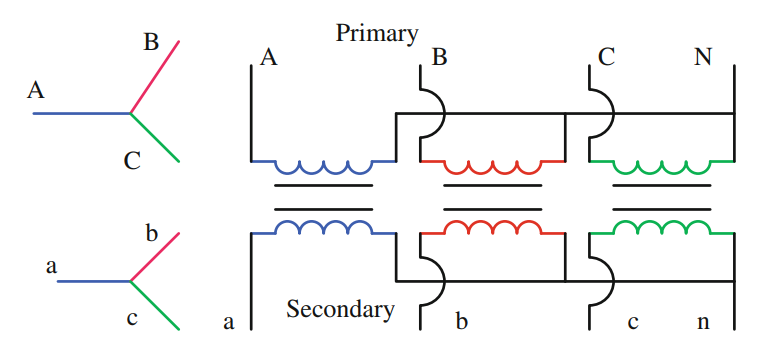
\includegraphics[scale=0.45]{graphics/Y_Y_Connection.PNG}
\caption{Y-Y connection diagram}
\end{figure}
\newpage
\item Y-$\Delta$ (wye-delta)
\begin{figure}[h!]
\center
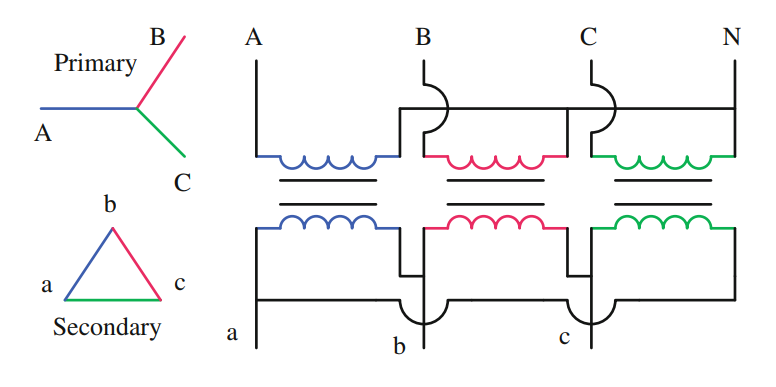
\includegraphics[scale=0.45]{graphics/Y_D_Connection.PNG}
\caption{Y-$\Delta$ connection diagram}
\end{figure}
\item $\Delta$- Y (delta-wye)
\begin{figure}[h!]
\center
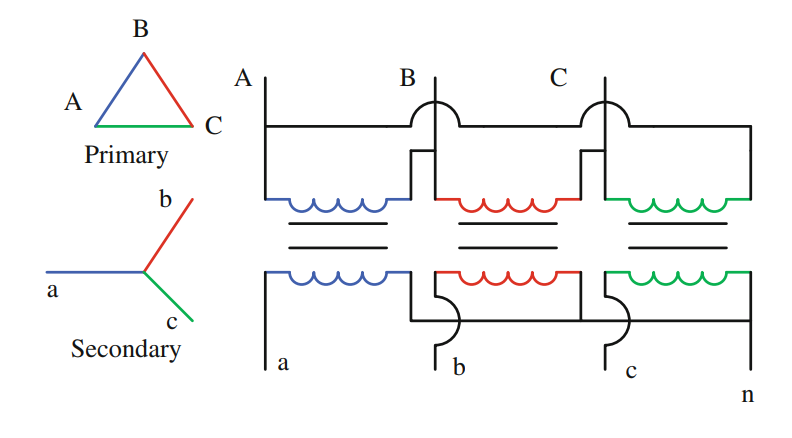
\includegraphics[scale=0.45]{graphics/D_Y_Connection.PNG}
\caption{$\Delta$-Y connection diagram}
\end{figure}
\item $\Delta$-$\Delta$ (delta - delta)
\begin{figure}[h!]
\center
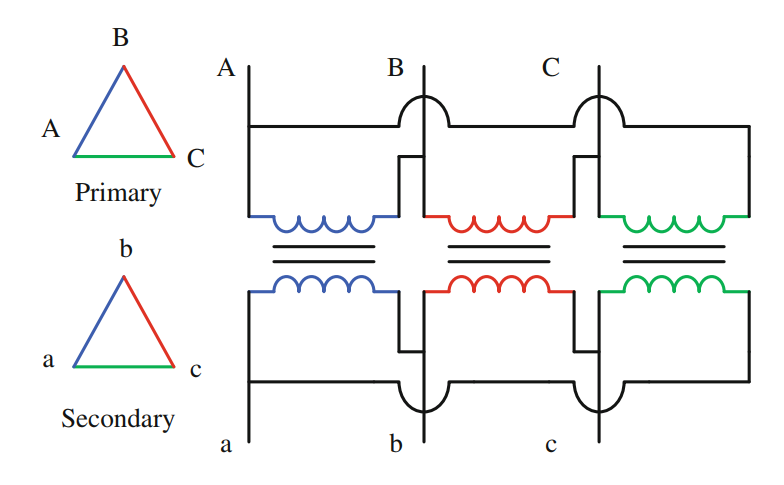
\includegraphics[scale=0.45]{graphics/D_D_Connection.PNG}
\caption{$\Delta$-$\Delta$ connection diagram}
\end{figure}
\end{itemize}  
The mainly used connection for a step down transformer is the Y-$\Delta$ (wye-delta) and for a step up is $\Delta$- Y (delta-wye)\cite{Salam_2016}[p. 88].
}{}

\section{Transformer Protection}
\ifdraft{
Since the transformer is very critical and expensive, the protection system needs to keep the transformer safe for operational use and here is listed some protective functions \cite{Constantin_2012}
\begin{itemize}\label{List: Transformer Protection systemms}
\itemsep0em 
\item Transformer Differential (87T)
\item Restricted earth fault or ground differential protection (87GN)
\item Instantaneous and inverse time Overcurrent (50$/$51)
\item Ground instantaneous and inverse time Overcurrent (50G/51G)
\item Current Unbalance/Negative Sequence (46)
\item Over-excitation (24)
\item Under-voltage (27)
\item Over-voltage (59)
\item Under-frequncy (81U)
\item Thermal Protection (49)
\item Breaker failure (50BF)
\end{itemize}
where the parenthesis numbers represent the ANSI device function.

\subsection{Transformer Differential (87T)}
Differential protection \cite{Trans_Diff87T} uses sensors on the primary and secondary connections that compares the two currents of the same phase.  If the currents equal each other than it is normal operation.  If the currents do not equal each other then the transformer is not in working correctly. The currents have amplitude difference between the primary and secondary because of phase difference because coupling in the transformer and ratio of current transformation.
The current matching of the primary winding is the same way of all vector shifts of the transformer.
\begin{equation}
\begin{split}
I_{1m} = \dfrac{I_{1p}}{ln(1)}- \dfrac{I_{1p}+I_{2p}+I_{3p}}{3ln(1)}\\
I_{2m} = \dfrac{I_{2p}}{ln(1)}- \dfrac{I_{1p}+I_{2p}+I_{3p}}{3ln(1)}\\
I_{3m} = \dfrac{I_{3p}}{ln(1)}- \dfrac{I_{1p}+I_{2p}+I_{3p}}{3ln(1)}\\
\end{split}
\end{equation} 
Where $I_{1m},I_{2m},I_{3m}$ is the matching value. $I_{1p},I_{2p},I_{3p}$ is the current value from the primary windings. See figure \ref{Fig: Vector shifts of transformer} for matching value for the second winding respective from vector shift. \cite{Trans_Diff87T}[p. 6]
\newpage
\begin{figure}[h!]
\center
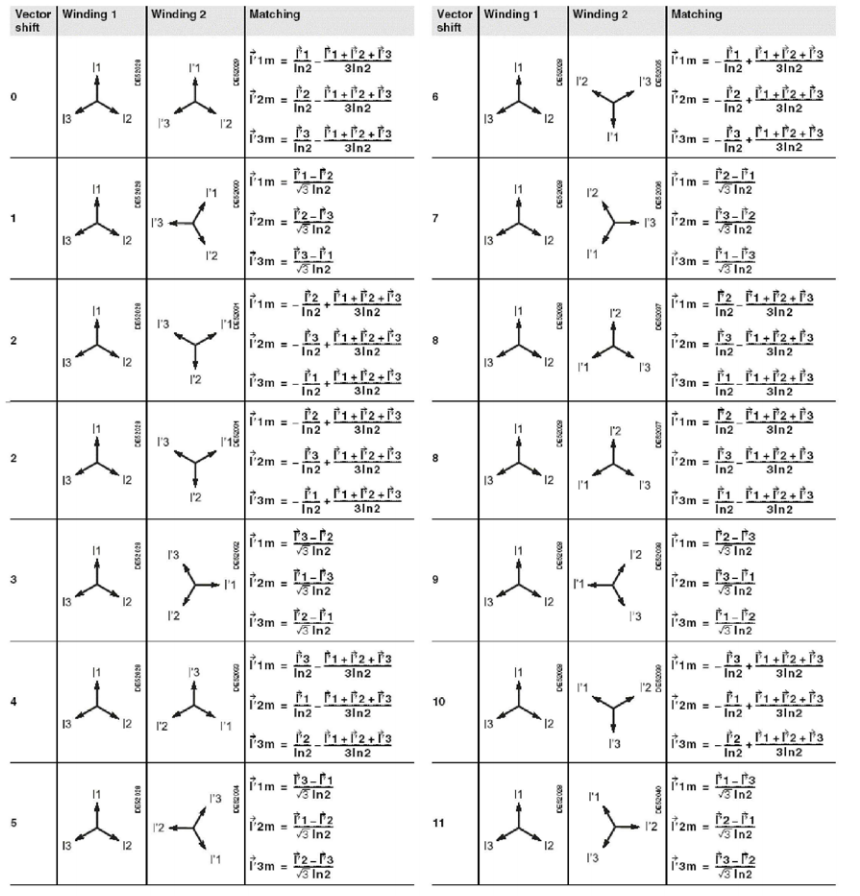
\includegraphics[scale=0.8]{graphics/Vector_Shift.png}
\caption{Vector Shifts of the Transformer with 123 type phase-rotation sequences}
\label{Fig: Vector shifts of transformer}
\end{figure}
}{}

\subsection{Restricted earth fault or ground differential protection (87GN)}
\ifdraft{The 87GN ground protection is sensitive enough to detect internal ground faults. It uses low-resistance grounded  .Fig \ref{Fig: Ground Differential Protection} shows the set up and is able to detect ground faults without false tripping on external faults \cite{Pillai_2004} \cite{Ramon_Ferran}.
\newpage
\begin{figure}[h!]
\center
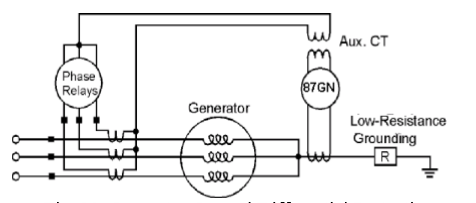
\includegraphics[scale=0.8]{graphics/Ground_Differential_Protection.PNG}
\caption{Ground Differential Protection}
\label{Fig: Ground Differential Protection}
\end{figure} 
}

\subsection{Ground instantaneous and inverse time Overcurrent (50G/51G)}
\ifdraft{
Figure \ref{Fig: Ground time and overcurrent protection} shows the set up for the 50G and 51G where they work together for using 50G overcurrent relays that are positioned on each feeder and using 51G inverse time overcurrent on the grounded neutral sources.  51G provideds protection against exernal faults if the 50G has not isolated the fault.  \cite{Pillai_2004} \cite{Ramon_Ferran}.
\begin{figure}[h!]
\center
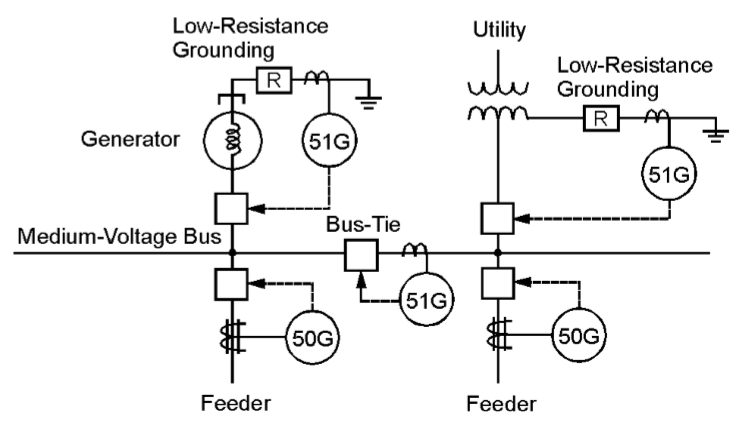
\includegraphics[scale=0.5]{graphics/Ground_Instantaneous_and_inverse_time_Overcurrent.PNG}
\caption{Ground time and overcurrent protection}
\label{Fig: Ground time and overcurrent protection}
\end{figure}

\subsection{Thermal Protection (49)}
When the transformer is turn on the electricity flows through it, the loss of power in the transformer is turned to heat.  

}

%\subsection{M-C system}

\subsection{Transformer fault}
\ifdraft{
The potential faults that happens in a transformer\\
Winding failure:
\begin{itemize}
\item turn-to-turn insulation failure
\item moisture
\item deterioration
\item phase-to-phase and ground faults
\item external faults (producing insulation failure
\end{itemize}
Tap changer failure:
\begin{itemize}
\item mechanical
\item electrical
\item short circuit
\item oil leak
\item overheating
\end{itemize}
Bushing failure:
\begin{itemize}
\item ageing, contamination and cracking
\item flash-over due to animals
\item moisture
\item low oil
\end{itemize}
Core failure:
\begin{itemize}
\item core insulation failure
\item ground strap burned away
\item loose clamps, bolts, wedges
\end{itemize}
Miscellaneous failure
\begin{itemize}
\item Bushing CT failure
\item metal particles in oil
\item damage in shipment
\item external faults
\item poor tank weld
\item over voltages
\item overloads
\end{itemize}
}

\subsection{Detection of transformer internal faults}
\ifdraft {
Phase-to-phase
\begin{itemize}
\item transformer differential protection
\item Buchholz relay
\item overpressure device
\item under-impedance/distance device
\item HV fuses
\end{itemize}
Ground-fault, low impedance
\begin{itemize}
\item restricted ground-fault protection
\item transformer differential protection
\item Buchholz relay
\item under-impedance/distance device
\item HV fuses
\end{itemize}
Ground-fault, high impedance grounding
\begin{itemize}
\item restricted ground-fault protection
\item sensitive ground-fault current protection
\item neutral (residual) over-voltage protection
\item Buchholz gas alarm
\end{itemize}
Turn-to-turn fault
\begin{itemize}
\item Buchholz alarm
\item transformer differential protection
\end{itemize}
HV to LV winding flash-over
\begin{itemize}
\item transformer differential protection
\item Buchholz relay
\item overpressure device (sudden pressure relay)
\end{itemize}

}

%%% Local Variables: 
%%% mode: latex
%%% TeX-master: "MSC-Kristján-2018"
%%% End: 
%% RUM: Literature Review 
%\chapter{Methods}

\lipsum[14-20]
%%% Local Variables: 
%%% mode: latex
%%% TeX-master: "DEGREE-NAME-YEAR"
%%% End: 
%%RUM: "Methods"
%\part{The Second Part}
%\chapter{Results}

In this section you discuss any issues that came up while developing
the system.  If you found something particularly interesting,
difficult, or an important learning experience, put it here.  This is
also a good place to put additional figures and data.

\lipsum[28-34]

%%% Local Variables: 
%%% mode: latex
%%% TeX-master: "DEGREE-NAME-YEAR"
%%% End: 
%%RUM: "Results"
%\chapter{Discussion}

\lipsum[35-41]

\section{Summary}
\lipsum[42-43]

\section{Conclusion\label{sec:conclusions}}
\lipsum[44-50]
%%% Local Variables: 
%%% mode: latex
%%% TeX-master: "DEGREE-NAME-YEAR"
%%% End: 
%%RUM: "Discussion"

%%%%%%%%% --------- REMEMBER %%%%%%%%------------------- %%%%%%%%%%

%% ---------------------------------------------------------------
\printbibliography{} %%RUM: "References"

%% If appendices are needed, uncomment the following line
%% and include the appendices in separate files
\appendix{}%%RUM: "Appendicies (as appropriate)
%\chapter{Code}\label{cha:code}
You can put code in your document using the listings package, which is
loaded by default in \path{custom.tex}.  Be aware that the listings
package does not put code in your document if you are in draft mode
unless you set the \texttt{forcegraphics} option.

There is an example java (Listing~\ref{src:Data_Bus.java}) and XML
file (Listing~\ref{src:AndroidManifest.xml}).  Thanks to the
\texttt{url} package, you can typeset OSX and unix paths like this:
\path{/afs/rnd.ru.is/project/thesis-template}.  Windows paths:
\path{C:\windows\temp\ }.  You can also typeset them using the menukey
package, but it tends to delete the last separator and has other
complications.\footnote{The menukey package has issues with biblatex,
  read \path{custom.tex} for more information.}

If you are trying to include multiple different languages, you should
go read the documentation and set these up in \path{custom.tex}.  You
will save yourself a lot of effort, especially if you have to fix
anything.

%I have put the source code in the \directory{src/} folder.
\lstinputlisting[language=Java, firstline=1,
lastline=40, caption={Data\_Bus.java: Setting up the class.},
label={src:Data_Bus.java}]{src/Data_Bus.java}

\lstinputlisting[language={[android]XML}, firstline=1, lastline=20,
caption={AndroidManifest.xml: Configuration for the Android UI.},
label={src:AndroidManifest.xml}]{src/AndroidManifest.xml}

%%% Local Variables: 
%%% mode: latex
%%% TeX-master: "DEGREE-NAME-YEAR"
%%% End: 
 % as an example, perhaps some of your code

%\backmatter{} % Sections after this don't get numbers
%% We prefer that all elements be numbered

%%%%%%%%%%%%% SHOW GLOSSARY %%%%%%%%%%%%%%%%%
%% Glossary, optional.  A good idea on longer documents
%% But it can cause problems with some LaTeX installations
%% without the morewrites package.  (which causes other problems)
%% Remember to run "makeglossaries <DEGREE-NAME-YEAR>"
%%   to update the glossary
%\printglossary{}%%RUM: Not mentioned
%\printacronyms{}%%RUM: Not mentioned

%% Glossary debugging code
%% Uncomment this to figure out of one of the glossary entries is broken
%% by putting all of the entries in the glossary.
%\ifthenelse{\boolean{debug}}{%
%  \glsaddall{} %put all entries in
%  \printglossaries{}}{}% dump them all
%% This command dumps all of the glossaries

%%%%%%%%%%%%% SHOW INDEX %%%%%%%%%%%%%%%%%%
%% Index, optional.  A good idea on longer documents

% You can put instructions at the beginning of the index:
%\renewcommand{\preindexhook}{%
%  The first page number is usually, but not always,
%  the primary reference to the indexed topic.\vskip\onelineskip}

%% You may have to run "makeindex <FILENAME>" to have it be generated
%% Depending upon which package you chose.
%% 
\clearforchapter{}
\printindex{}%%RUM: Not mentioned

\backcover{}%%RUM: "Back cover (standard)
\end{document}

%% ---------------------------------------------------------------

%%%%%%%%%%%%%%%%%%%% TeXStudio Magic Comments %%%%%%%%%%%%%%%%%%%%%
%% These comments that start with "!TeX" modify the way TeXStudio works
%% For details see http://texstudio.sourceforge.net/manual/current/usermanual_en.html   Section 4.10
%%
%% What encoding is the file in?
% !TeX encoding = UTF-8
%% What language should it be spellchecked?
% !TeX spellcheck = en_US
%% What program should I compile this document with?
% !TeX program = pdflatex
%% Which program should be used for generating the bibliography?
% !TeX TXS-program:bibliography = txs:///biber
%% This also sets the bibliography program for TeXShop and TeXWorks
% !BIB program = biber

%%% Local Variables:
%%% mode: latex
%%% TeX-master: t
%%% End:
